\documentclass[11pt, oneside]{article}
\usepackage[letterpaper, margin=2cm]{geometry}
\usepackage{MATH566}
%\usepackage{sagetex}

\begin{document}
\noindent \textbf{\Large{Caleb Logemann \\
MATH 566 Discrete Optimization\\
Final
}}

%\lstinputlisting[language=Sage]{03_2.sage}
\begin{enumerate}
  \item % #1 Done
    Emperor has decided to build Death Star II.
    He needs  money to pay for it.
    He sent you to collect taxes from several planets.
    Here are the coordinates of the planets assigned to you.
    You are starting at Corusant (0,0) and want to return there.
    The time of travel between the planets corresponds to their Euclidean
    distance.
    You have to visit all planets.
    Minimize the travel time.
    \begin{verbatim}
      X = [  [0,0], [9,0], [1,1], [8,1], [0,2], [9,2], [4,3], [5,3], \
      [0,4], [1,4], [2,4], [3,4], [6,4], [7,4], [8,4], [9,4], \
      [0,5], [1,5], [3,5], [2,5], [6,5], [7,5], [8,5], [9,5], \
      [4,6], [5,6], [0,7], [9,7], [1,8], [8,8], [0,9], [9,9] ];
    \end{verbatim}

    This is a traveling salesman problem.
    There are several approximation algorithms that can find good solutions.
    I have programmed the nearest neighbor algorithm, the cheapest insertion
    algorithm, and the furthest insertion algorithm in the following script.
    This script also has a function to compute a lower bound on the traveling
    salesman tour.
    \lstinputlisting[language=Sage]{Sage/travelingSalesman.sage}
    The lower bound function uses Kruskal's algorithm to find the minimum spanning tree.
    This algorithm is implemented below.
    \lstinputlisting[language=Sage]{Sage/kruskal.sage}
    The following script runs each of these algorithms on the given set of
    points and computes a lower bound.
    \lstinputlisting[language=Sage]{Sage/final_1.sage}
    The output of this script is shown below.
    \begin{verbatim}
      Nearest Neighbor
      Distance: 65.0902577378837
      Cheapest Insertion
      Distance: 63.3137084989848
      Furthest Insertion
      Distance: 55.0364766805865
      Lower Bound: 40.7279220613579
    \end{verbatim}
    The following plots are also generated.
    For the nearest neighbor algorithm the following tour was found.
    \begin{center}
      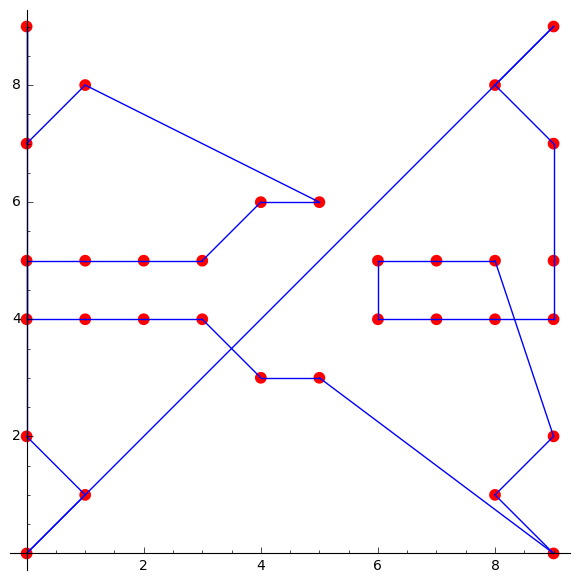
\includegraphics[scale=.5]{Figures/final_1.png}
    \end{center}
    For the cheapest insertion algorithm the following tour was found.
    \begin{center}
      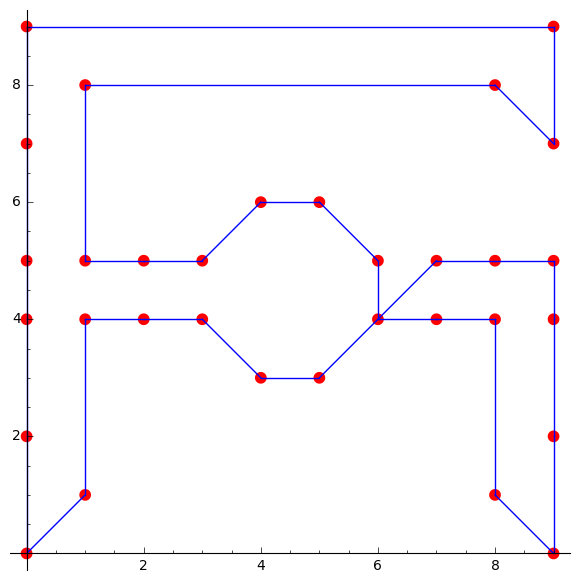
\includegraphics[scale=.5]{Figures/final_2.png}
    \end{center}
    For the furthest insertion algorithm the following tour was found.
    \begin{center}
      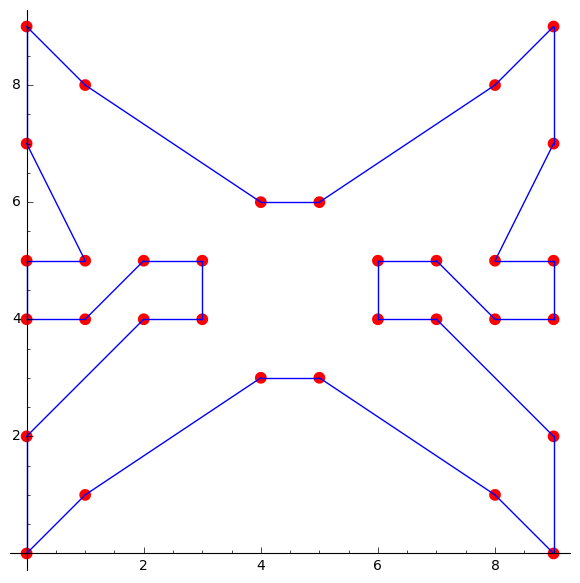
\includegraphics[scale=.5]{Figures/final_3.png}
    \end{center}
    The furthest insertion algorithm found the best tour out of all three
    algorithms with a total distance of 55.036.
    The lower bound that was found was 40.728.

  \item % #2 Done
    You are leading a group $4$ of imperial fighters that are protecting an
    imperial shuttle transporting secret plans to Death Star II. 
    You were ambushed by $3$ rebel ships.
    You must protect the secret plans!
    Do not repeat the same mistake that happened with Death Star.

    Choose one fighter from your group to accompany the transport shuttle cover
    their retreat by fighting the rebel ship.
    The remaining three ships will each try to fight one rebel ship.
    You need to fight against each of the rebel ships to prevent pursuit of the
    transport shuttle and you do not want to leave the transport ship unguarded.

    For the remaining 3 ships that fight the rebel ships, maximize the total
    damage (sum of damages) caused to the rebel ships.
    For every pair of imperial and rebel ship, the damage caused by imperial
    ships to rebel ships is described in the following table.
    \begin{center}
      \begin{tabular}{c|ccccc}
              & $r_1$ & $r_2$ & $r_3$ \\ \hline
        $i_1$ &    3  &     2 &     3 \\
        $i_2$ &    2  &     3 &     1 \\
        $i_3$ &    4  &     2 &     2 \\
        $i_4$ &    1  &     5 &     1 \\
      \end{tabular}
    \end{center}

    This problem can be solved using an integer program.
    Let $x_{ir} \in \set{0, 1}$ be a variable describing whether imperial ship
    $i$ is going to attach rebel ship $r$.
    The damage that imperial ship $i$ can cause to rebel ship $r$ will be given
    by $d_{ir}$.
    These values are constant and are given in the table above.
    Therefore the objective function for this integer program will be
    \[
      \text{maximize } \sum{i = 1}{4}{\sum{r = 1}{3}{d_{ir} x_{ir}}}
    \]
    There are several constraints on the variables $x_{ir}$.
    The first constraint is each imperial ship can attach at most one rebel ship,
    that is
    \[
      \sum{r = 1}{3}{x_{ir}} \le 1 \text{ for } 1 \le i \le 4
    \]
    Also every rebel ship must be attacked by at least one imperial ship.
    \[
      \sum{i = 1}{4}{x_{ir}} \ge 1 \text{ for } 1 \le r \le 3
    \]
    Lastly one ship must guard the transport ship, or in other words at most
    three imperial ships can attack the rebel ships.
    \[
      \sum{i = 1}{4}{\sum{r = 1}{3}{x_{ir}}} \le 3
    \]

    The full integer program is thus
    \[
      (IP)
      \begin{cases}
        \text{maximize} & \sum{i = 1}{4}{\sum{r = 1}{3}{d_{ir} x_{ir}}} \\
        \text{subject to} & \sum{r = 1}{3}{x_{ir}} \le 1 \text{ for } 1 \le i \le 4 \\
                          & \sum{i = 1}{4}{x_{ir}} \ge 1 \text{ for } 1 \le r \le 3 \\
                          & \sum{i = 1}{4}{\sum{r = 1}{3}{x_{ir}}} \le 3 \\
                          & x_{ir} \in \set{0, 1} \quad \forall i, r
      \end{cases}
    \]
    The following Sage script implements this integer program.
    \lstinputlisting[language=Sage]{Sage/final_2.sage}
    The output of this script is shown below.
    \begin{verbatim}
      Objective Value: 12.0
      x[(1, 2)] = 0.0
      x[(3, 2)] = 0.0
      x[(1, 3)] = 1.0
      x[(3, 3)] = 0.0
      x[(3, 1)] = 1.0
      x[(2, 1)] = 0.0
      x[(2, 3)] = 0.0
      x[(4, 3)] = 0.0
      x[(2, 2)] = 0.0
      x[(4, 2)] = 1.0
      x[(4, 1)] = 0.0
      x[(1, 1)] = 0.0
    \end{verbatim}

  \item % #3 Done
    Darth Vader forgot his lightsaber.
    Bring it to him as fast as you can so the Emperor can watch a lightsaber
    fight between Darth Vader and Luke Skywalker.
    You have only a small ship and hence you need refueling.
    Here is a map of the space.
    Every planet has a number that corresponds to the time needed for refueling 
    and every connection has a travel time associated to it. 

    \begin{center}
      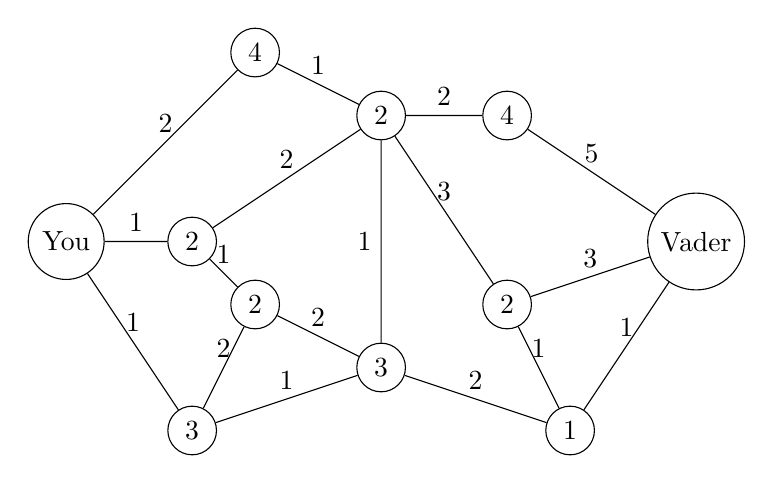
\begin{tikzpicture}[scale=0.8]
        \draw (0,0) node[circle,draw](y){You};
        \draw (10,0) node[circle,draw](v){Vader};
        \draw (2,-3) node[circle,draw](p1){3};
        \draw (3,3) node[circle,draw](p2){4};
        \draw (2,0) node[circle,draw](p3){2};
        \draw (5,-2) node[circle,draw](p4){3};
        \draw (5,2) node[circle,draw](p5){2};
        \draw (3,-1) node[circle,draw](p6){2};
        \draw (7,2) node[circle,draw](p7){4};
        \draw (7,-1) node[circle,draw](p8){2};
        \draw (8,-3) node[circle,draw](p9){1};
        \draw
          (y) -- node[above]{1} (p1)
          (y) -- node[above]{2} (p2)
          (y) -- node[above]{1} (p3)
          (p1) -- node[above]{1} (p4)
          (p1) -- node[above]{2} (p6)
          (p3) -- node[above]{1} (p6)
          (p3) -- node[above]{2} (p5)
          (p2) -- node[above]{1} (p5)
          (p5) -- node[above]{2} (p7)
          (p5) -- node[above]{3} (p8)
          (p5) -- node[left]{1} (p4)
          (p4) -- node[above]{2} (p6)
          (p4) -- node[above]{2} (p9)
          (p8) -- node[above]{1} (p9)
          (p8) -- node[above]{3} (v)
          (p9) -- node[above]{1} (v)
          (p7) -- node[above]{5} (v)
        ; 
      \end{tikzpicture}
    \end{center}

    This is a shortest path problem with the addition of weights on the
    vertices.
    This problem can be solved with a slightly modified version of Djikstra's
    algorithm.
    Note that Dijkstras algorithm will work because all edge and vertex weights
    are positive.

    In order to handle the vertex weights as well a couple of modifications are
    necessary.
    First the distance from the source to itself should be the weight of the source
    vertex instead of zero.
    In our case the weight of the source is zero anyways.
    Second when modifying the distance from the source to any other vertex the
    weight of the target vertex must also be included.
    For example if attempting to add edge $(v, w)$, normally the following
    occurs
    \[
      l(w) = \min{l(w), l(v) + c(v, w)}
    \]
    where $c(v, w)$ is the cost of the $(v, w)$ edge.
    With the addition of vertex weights the following update will occur.
    \[
      l(w) = \min{l(w), l(v) + c(v, w) + c(w)}
    \]
    where $c(w)$ is the cost of the vertex $w$.
    Note that $l(v)$ will already have the cost of $v$ accounted for.
    These two modifications will allows Dijkstra's Algorithm to solve this
    problem.

    The following function runs Dijkstra's Algorithm with the forementioned
    modifications.
    \lstinputlisting[language=Sage]{Sage/dijkstras.sage}
    Now I will label the vertices of the graph as follows, while keeeping
    in mind the weights on the vertices
    \begin{center}
      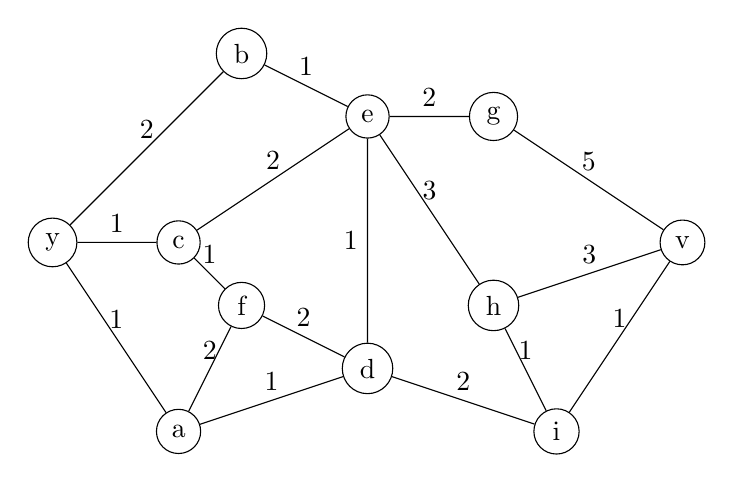
\begin{tikzpicture}[scale=0.8]
        \draw (0,0) node[circle,draw](y){y};
        \draw (10,0) node[circle,draw](v){v};
        \draw (2,-3) node[circle,draw](p1){a};
        \draw (3,3) node[circle,draw](p2){b};
        \draw (2,0) node[circle,draw](p3){c};
        \draw (5,-2) node[circle,draw](p4){d};
        \draw (5,2) node[circle,draw](p5){e};
        \draw (3,-1) node[circle,draw](p6){f};
        \draw (7,2) node[circle,draw](p7){g};
        \draw (7,-1) node[circle,draw](p8){h};
        \draw (8,-3) node[circle,draw](p9){i};
        \draw
          (y) -- node[above]{1} (p1)
          (y) -- node[above]{2} (p2)
          (y) -- node[above]{1} (p3)
          (p1) -- node[above]{1} (p4)
          (p1) -- node[above]{2} (p6)
          (p3) -- node[above]{1} (p6)
          (p3) -- node[above]{2} (p5)
          (p2) -- node[above]{1} (p5)
          (p5) -- node[above]{2} (p7)
          (p5) -- node[above]{3} (p8)
          (p5) -- node[left]{1} (p4)
          (p4) -- node[above]{2} (p6)
          (p4) -- node[above]{2} (p9)
          (p8) -- node[above]{1} (p9)
          (p8) -- node[above]{3} (v)
          (p9) -- node[above]{1} (v)
          (p7) -- node[above]{5} (v)
        ; 
      \end{tikzpicture}
    \end{center}
    Now the following script will run the algorithm on this graph.
    \lstinputlisting[language=Sage]{Sage/final_3.sage}
    The output of this script is as follows.
    \begin{verbatim}
      Distance: 12
      Shortest path: ['y', 'a', 'd', 'i', 'v']
    \end{verbatim}
    So the shortest path from me to Vader is of length 12 and is marked in
    the graph below.
    \begin{center}
      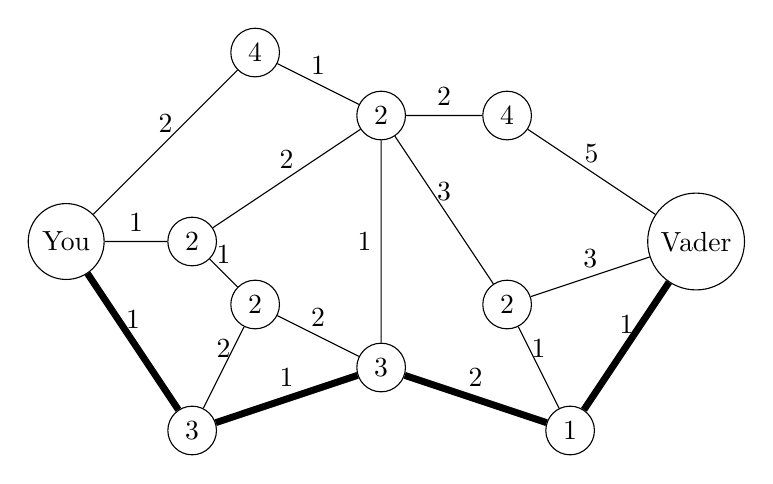
\begin{tikzpicture}[scale=0.8]
        \draw (0,0) node[circle,draw](y){You};
        \draw (10,0) node[circle,draw](v){Vader};
        \draw (2,-3) node[circle,draw](p1){3};
        \draw (3,3) node[circle,draw](p2){4};
        \draw (2,0) node[circle,draw](p3){2};
        \draw (5,-2) node[circle,draw](p4){3};
        \draw (5,2) node[circle,draw](p5){2};
        \draw (3,-1) node[circle,draw](p6){2};
        \draw (7,2) node[circle,draw](p7){4};
        \draw (7,-1) node[circle,draw](p8){2};
        \draw (8,-3) node[circle,draw](p9){1};
        \draw
          (y) -- node[above]{2} (p2)
          (y) -- node[above]{1} (p3)
          (p1) -- node[above]{2} (p6)
          (p3) -- node[above]{1} (p6)
          (p3) -- node[above]{2} (p5)
          (p2) -- node[above]{1} (p5)
          (p5) -- node[above]{2} (p7)
          (p5) -- node[above]{3} (p8)
          (p5) -- node[left]{1} (p4)
          (p4) -- node[above]{2} (p6)
          (p8) -- node[above]{1} (p9)
          (p8) -- node[above]{3} (v)
          (p7) -- node[above]{5} (v)
        ; 
        \draw[line width=2.5pt]
          (y) -- node[above]{1} (p1)
          (p1) -- node[above]{1} (p4)
          (p4) -- node[above]{2} (p9)
          (p9) -- node[above]{1} (v)
        ;
      \end{tikzpicture}
    \end{center}

  \item % #4 Done
    The Emperor, as any other good emperor, knows that it is best if his enemies
    are fighting among each other.
    Here is a map of Emperor's enemies and how much does it cost for each pair
    to start fighting each other.
    Find for the Emperor which pairs to trick into fighting each other such that
    every enemy is in exactly one fight.
    Provide also a certificate verifying the optimality of your solution.\\

    \begin{center}
      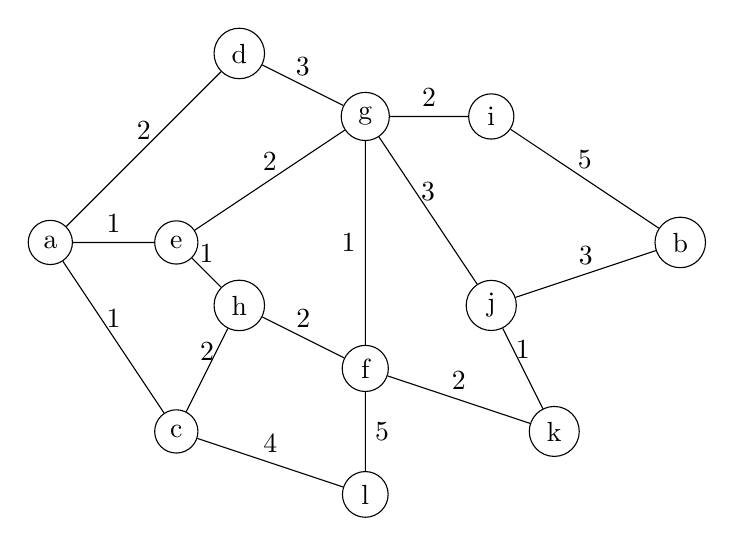
\begin{tikzpicture}[scale=0.8]
        \draw (0,0) node[circle,draw](y){a};
        \draw (10,0) node[circle,draw](v){b};
        \draw (2,-3) node[circle,draw](p1){c};
        \draw (3,3) node[circle,draw](p2){d};
        \draw (2,0) node[circle,draw](p3){e};
        \draw (5,-2) node[circle,draw](p4){f};
        \draw (5,2) node[circle,draw](p5){g};
        \draw (3,-1) node[circle,draw](p6){h};
        \draw (7,2) node[circle,draw](p7){i};
        \draw (7,-1) node[circle,draw](p8){j};
        \draw (8,-3) node[circle,draw](p9){k};
        \draw (5,-4) node[circle,draw](p10){l};
        \draw
          (y) -- node[above]{1} (p1)
          (y) -- node[above]{2} (p2)
          (y) -- node[above]{1} (p3)
          (p1) -- node[above]{2} (p6)
          (p3) -- node[above]{1} (p6)
          (p3) -- node[above]{2} (p5)
          (p2) -- node[above]{3} (p5)
          (p5) -- node[above]{2} (p7)
          (p5) -- node[above]{3} (p8)
          (p5) -- node[left]{1} (p4)
          (p4) -- node[above]{2} (p6)
          (p4) -- node[above]{2} (p9)
          (p8) -- node[above]{1} (p9)
          (p8) -- node[above]{3} (v)
          (p7) -- node[above]{5} (v)
          (p4) -- node[right]{5} (p10)
          (p1) -- node[above]{4} (p10)
        ; 
      \end{tikzpicture}
    \end{center}

    This is a minimum matching problem in a weighted bipartite graph.
    To see that this graph is bipartite note that the vertices can be
    partitioned into sets $\set{a, b, g, h, k, l}$ and
    $\set{c, d, e, f, i, j}$, that are not internally connected.
    The minimum matching problem in a weighted bipartite graph can be solved
    with the following integer program.
    \[
      (IP)
      \begin{cases}
        \text{maximize} & \sum{e \in E}{}{c(e)x_e} \\
        \text{subject to} & \sum{e \in \delta(v)}{}{x_e} = 1 \quad \forall v \in V \\
                          & x_e \in \set{0, 1} \quad \forall e \in E
      \end{cases}
    \]
    where $x_e$ represent whether edge $e$ is in the matching.

    The following script implements this integer program for the given graph
    in Sage.
    \lstinputlisting[language=Sage, lastline=30]{Sage/final_4.sage}
    The output of the script is shown below.
    \begin{verbatim}
      Objective Value: 14.0
      x[('j', 'k', 1)] = 0.0
      x[('a', 'd', 2)] = 1.0
      x[('g', 'j', 3)] = 0.0
      x[('a', 'e', 1)] = 0.0
      x[('d', 'g', 3)] = 0.0
      x[('c', 'l', 4)] = 1.0
      x[('e', 'g', 2)] = 0.0
      x[('f', 'k', 2)] = 1.0
      x[('b', 'i', 5)] = 0.0
      x[('f', 'l', 5)] = 0.0
      x[('c', 'h', 2)] = 0.0
      x[('b', 'j', 3)] = 1.0
      x[('f', 'h', 2)] = 0.0
      x[('a', 'c', 1)] = 0.0
      x[('g', 'i', 2)] = 1.0
      x[('e', 'h', 1)] = 1.0
      x[('f', 'g', 1)] = 0.0
    \end{verbatim}
    The matching can be viewed in the graph as follows.
    \begin{center}
      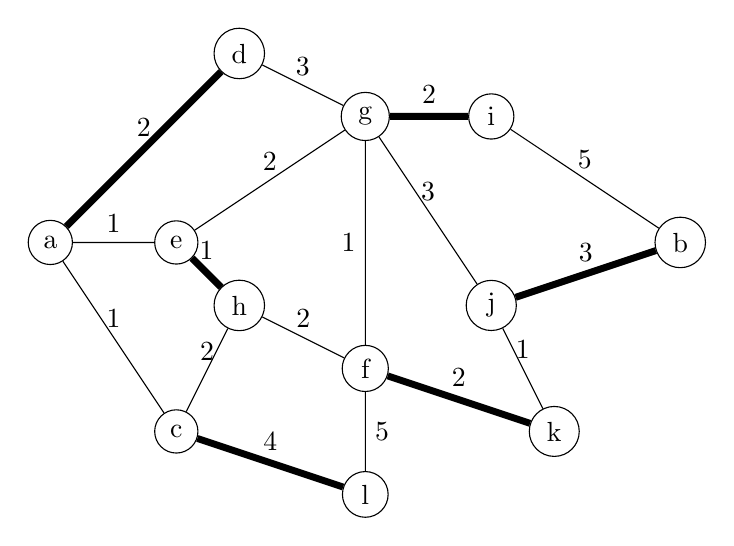
\begin{tikzpicture}[scale=0.8]
        \draw (0,0) node[circle,draw](a){a};
        \draw (10,0) node[circle,draw](b){b};
        \draw (2,-3) node[circle,draw](c){c};
        \draw (3,3) node[circle,draw](d){d};
        \draw (2,0) node[circle,draw](e){e};
        \draw (5,-2) node[circle,draw](f){f};
        \draw (5,2) node[circle,draw](g){g};
        \draw (3,-1) node[circle,draw](h){h};
        \draw (7,2) node[circle,draw](i){i};
        \draw (7,-1) node[circle,draw](j){j};
        \draw (8,-3) node[circle,draw](k){k};
        \draw (5,-4) node[circle,draw](l){l};
        \draw
          (a) -- node[above]{1} (c)
          (a) -- node[above]{1} (e)
          (c) -- node[above]{2} (h)
          (e) -- node[above]{2} (g)
          (d) -- node[above]{3} (g)
          (g) -- node[above]{3} (j)
          (g) -- node[left]{1} (f)
          (f) -- node[above]{2} (h)
          (j) -- node[above]{1} (k)
          (i) -- node[above]{5} (b)
          (f) -- node[right]{5} (l)
        ; 
        \draw[line width=2.5pt]
          (a) -- node[above]{2} (d)
          (c) -- node[above]{4} (l)
          (f) -- node[above]{2} (k)
          (j) -- node[above]{3} (b)
          (g) -- node[above]{2} (i)
          (e) -- node[above]{1} (h)
        ;
      \end{tikzpicture}
    \end{center}

    In order to check that this is in fact the optimal solution the dual linear
    program can be solved as well.
    If the provide the same optimal value, then we know that we have found
    an optimal solution.
    The dual integer program is
    \[
      (D)
      \begin{cases}
        \text{maximize} & \sum{v \in V}{}{y_v} \\
        \text{subject to} & y_u + y_v \le c(u,v) \quad \forall (u, v) \in E \\
                          & y_v \in \RR \quad \forall v \in V
      \end{cases}
    \]

    The following script implements this linear program for the given graph.
    \lstinputlisting[language=Sage, firstline=32]{Sage/final_4.sage}
    The output of this script is shown below.
    \begin{verbatim}
      Objective Value: 14.0
      y[a] = -0.0
      y[c] = 1.0
      y[b] = 3.0
      y[e] = 1.0
      y[d] = 2.0
      y[g] = 0.0
      y[f] = 1.0
      y[i] = 2.0
      y[h] = 0.0
      y[k] = 1.0
      y[j] = 0.0
      y[l] = 3.0
    \end{verbatim}
    As shown the optimal solution has value 14 just as the original program did.
    This shows that we have in fact found an optimal solution.
\end{enumerate}
\end{document}
